\documentclass{exam}
\input{../preamble}
\pagestyle{headandfoot}
\firstpageheader{Physics}{Unit 2: Acceleration}{Test}

\CorrectChoiceEmphasis{\color{red}\bfseries}
\SolutionEmphasis{\color{red}}
\printanswers




\begin{document}

\begin{center}
\fbox{\fbox{\parbox{5.5in}{\centering USEFUL INFORMATION
\begin{equation*}
    a = \frac{\Delta{v}}{\Delta{t}} = \frac{v_f - v_0}{t_f - t_0} \quad\quad \SI{1}{km} = \SI{1000}{m} \quad\quad \SI{1}{h} = \SI{60}{min} \quad\quad \SI{1}{min} = \SI{60}{s}
\end{equation*}
}}}
\end{center}
\begin{questions}



\question
A rock is dropped from rest from the top of a tall cliff, taking \SI{5.0}{s} to reach the ground. If the rock impacts the ground at a velocity of \SI{49}{m/s}, what is the acceleration due to gravity?

\begin{choices}
    \choice \SI{0.10}{m/s^2}
    \correctchoice \SI{9.8}{m/s^2}
    \choice \SI{4.9}{m/s^2}
    \choice \SI{245}{m/s^2}
\end{choices}

\question
If an object's acceleration is \SI{3}{m/s^2}, then with every second that passes, the object's velocity (speed) will increase by \fillin[][2cm]\ .

\begin{choices}
    \choice \SI{1}{m/s}
    \choice \SI{2}{m/s}
    \correctchoice \SI{3}{m/s}
    \choice \SI{4}{m/s}
\end{choices}

\question
Jasmine starts from rest and accelerates her bicycle at \SI{3}{m/s^2}. What will be her velocity after 4 seconds?

\begin{choices}
    \choice \SI{0.083}{m/s}
    \choice \SI{0.75}{m/s}
    \choice \SI{1.3}{m/s}
    \correctchoice \SI{12}{m/s}
\end{choices}

\question
What are the units used to measure acceleration?

\begin{choices}
    \choice meters per second (\SI{}{m/s})
    \correctchoice meters per second squared (\SI{}{m/s^2})
    \choice meters (m)
    \choice seconds (s)
\end{choices}

\clearpage
\question %This problem and the next one go together.
A subway train accelerates from rest to \SI{12.8}{m/s} (\SI{45.9}{km/h}) in \SI{17.0}{s}. What is the average acceleration during that time interval?

\begin{choices}
\choice \SI{12.8}{m/s}
\choice \SI{2.70}{m/s^2}
\choice \SI{45.9}{m/s^2}
\CorrectChoice \SI{0.753}{m/s^2} 
\end{choices}

\question 
%Relating the result of this problem (train's velocity at 17 s) to the previous counterpart created epiphanies for serveral students. When we showed that we arrive at the final velocity from the previous problem (12.8 m/s), some students went "Ohh, that's really cool!"
A train starting from rest accelerates at \SI{0.753}{m/s^2}. Complete the table below, calculating changes in the train's velocity across time.

\begin{figure}[h!]
    \centering
    \begin{tabular}{c|c}
        \textbf{Time (s)} & \textbf{Velocity (m/s)} \\
        \hline
        0 & 0\\
        1 &  \\
        2 &  \\
        3 &  \\
        4 &  \\
        \vdots &  \\
        17 &  \\
    \end{tabular}
\end{figure}

\question
Coco the dog trots at \SI{2.0}{m/s}. When she hears her owner say ``Treat!'' she accelerates at \SI{1.2}{m/s^2} for \SI{4.0}{s}. What is Coco's final velocity?

\begin{choices}
    \choice \SI{4.8}{m/s}
    \correctchoice \SI{6.8}{m/s}
    \choice \SI{2.0}{m/s}
    \choice \SI{1.2}{m/s}
\end{choices}

John is cruising in his car at \SI{35}{m/s} when the traffic light turns yellow, causing him to momentarily to hit the breaks. If he decelerates at \SI{-10}{m/s}, what will be his final velocity after \SI{3}{seconds}?

\begin{choices}
    \correctchoice \SI{}{m/s}
\end{choices}

\question
An object accelerates from \SI{120}{m/s} to \SI{145}{m/s} at a rate of \SI{7.5}{m/s^2}. How long will it take the object to reach its final velocity?

\begin{choices}
    \correctchoice \SI{3.3}{s}
    \choice \SI{4.9}{s}
    \choice \SI{0.3}{s}
    \choice \SI{25}{s}
\end{choices}

\clearpage
\question
The Houston Zoo releases a falcon from a cage. The falcon flies at \SI{5}{m/s}. When it sees its breakfast (a small mouse), it accelerates to \SI{32}{m/s} in \SI{7.2}{s}. What is the falcon's average acceleration?
%$a = \SI{3.75}{m/s^2}$

\question
Hurricane Iris crosses Cuba at \SI{5.0}{m/s}. When it reaches the ocean, it accelerates at \SI{0.48}{m/s^2} for \SI{35}{s}. What will be Hurricane Iris's final velocity?

\question 
Tom rides in a jet that accelerates from \SI{53.6}{m/s} to \SI{134}{m/s} at a rate of \SI{26.8}{m/s^2}. How long will it take Tom to reach his top velocity?


\question
What is acceleration?

\begin{choices}
\choice The rate of change of acceleration.
\choice The rate of change of position. 
\CorrectChoice The rate of change of velocity.
\choice The rate of change of time.
\end{choices}

\question %Like PCA
An elevator moves downward as its speed \textit{decreases}. What is the direction of its acceleration?

\begin{choices}
\choice Left
\choice Right 
\correctchoice Up
\choice Down
\end{choices}

\question %Like PCA
A car travels eastward as its speed \textit{increases}. What is the direction of its acceleration?

\begin{choices}
\choice North
\choice South 
\correctchoice East
\choice West
\end{choices}


\question % Like Ch2 #16
A cheetah can accelerate from rest to a speed of 
\SI{35.0}{m/s}
in 
\SI{7.00}{s}
. What is its acceleration?

\begin{choices}
\choice \SI{245}{m/s^2}
\choice \SI{0.309}{m/s^2}
\CorrectChoice \SI{5.00}{m/s^2}
\choice \SI{18.2}{m/s^2}
\end{choices}

\question % Like Ch2 #18
A commuter backs her car out of her garage with an acceleration of \SI{1.2}{m/s^2}. How long does it take her to reach a speed of \SI{2.4}{m/s}?

\begin{choices}
\choice \SI{2.9}{s}
\correctchoice \SI{2.0}{s}
\choice \SI{0.5}{s}
\choice \SI{3.6}{s}
\end{choices}


% \begin{choices}
% \choice \SI{6.9}{s}
% \choice \SI{1.5}{s}
% \CorrectChoice \SI{1.3}{s}
% \choice \SI{0.22}{s}
% \end{choices}

\question %Like OpenStax Physics Ch2 #8 https://openstax.org/books/physics/pages/3-critical-thinking-items

A motorcycle moving at a constant velocity suddenly accelerates at a rate of \SI{3.0}{m/s^2} to a speed of \SI{30}{m/s} in \SI{4.0}{s}. What was the initial speed of the motorcycle?

\begin{choices}
\choice \SI{0.0}{m/s}
\choice \SI{10}{m/s}
\choice \SI{12}{m/s}
\CorrectChoice \SI{18}{m/s}
\end{choices}

\question %Like Example 2.10 
Dragsters can achieve average accelerations of \SI{24.0}{m/s^2}. Suppose such a dragster accelerates from rest at this rate for \SI{4.00}{s}. How far does it travel in this time?

\begin{choices}
\choice \SI{48.0}{m}
\choice \SI{96.0}{m}
\correctchoice \SI{192}{m}
\choice \SI{6.00}{m}
\end{choices}

% \begin{solution}

% $a = \SI{24.0}{m/s^2}$, $v_0 = 0$, $t = \SI{4.00}{s}$. Let $x_0 = 0$

% $x =\ ?$

% \begin{equation*}
%     x = x_0 + v_0 t + \frac{1}{2} a t^2 = \SI{192}{m}
% \end{equation*}
% \end{solution}


%\clearpage
\question %Like Ch2 #27
In a slap shot, a hockey player accelerates the puck from a velocity of \SI{5.0}{m/s} to \SI{85}{m/s} in the same direction. If this shot takes \SI{7.0e-2}{s}, calculate the distance over which the puck accelerates.

\begin{choices}
\choice \SI{0.35}{m}
\correctchoice \SI{2.8}{m}
\choice \SI{5.9}{m}
\choice \SI{5.6}{m}
\end{choices}

% \begin{solution}
% $v_0 = \SI{5.0}{m/s}$, $v = \SI{85}{m/s}$, $t = \SI{7.0e-2}{s}$. Let $x_0 = 0$.

% $x =\ ?$

% The average velocity is

% \begin{equation*}
%     \bar{v} = \frac{v_0 + v}{2} = \SI{40}{m/s}\ .
% \end{equation*}

% Therefore, distance traveled is

% \begin{equation*}
%     x = x_0 + \bar{v}t = \SI{2.8}{m}\ .
% \end{equation*}
% \end{solution}

\clearpage
\begin{EnvUplevel}
\textbf{For Questions \ref{prob:cliff_rock1} through \ref{prob:cliff_rock3}, refer to the passage below.}

A person standing on the edge of a high cliff throws a rock straight up with an initial velocity of 13.0 m/s. The rock misses the edge of the cliff as it falls back to earth.

Assume that \textit{up} is the positive direction and that air resistance is negligible.
\end{EnvUplevel}%Like Example 2.14

\question \label{prob:cliff_rock1}
What is the rock's acceleration after 10 seconds of motion? ($g = \SI{9.8}{m/s^2}$)

\begin{choices}
\choice $a = g$
\choice $a < g$
\correctchoice $a = -g$
\choice $a > g$
\end{choices}

\question \label{prob:cliff_rock2}
Calculate the \textbf{position} of the rock \SI{2.3}{s} after it is thrown. Assume the initial position is zero.

\begin{choices}
\correctchoice \SI{4.0}{m}
\choice \SI{29.9}{m}
\choice \SI{5.6}{m}
\choice \SI{15.3}{m}
\end{choices}

\question \label{prob:cliff_rock3}
What is the \textbf{velocity} of the rock \SI{5.0}{s} after it is thrown?

\begin{choices}
\correctchoice \SI{-36}{m/s}
\choice \SI{-13}{m/s}
\choice \SI{0}{m/s}
\choice \SI{65}{m/s}
\end{choices}

\vspace{1em}
\hrule

\question %Like Ch2 #33
An unwary football player collides with a padded goalpost while running at a velocity of \SI{7.0}{m/s} and comes to a full stop after compressing the padding and his body \SI{0.50}{m}. What is his deceleration?

\begin{choices}
\choice \SI{-3.5}{m/s^2}
\choice \SI{-14}{m/s^2}
\correctchoice \SI{-49}{m/s^2}
\choice \SI{-9.8}{m/s^2}
\end{choices}

% \begin{solution}

% $v_0 = \SI{7.0}{m/s}$, $v = 0$, $\Delta{x} = x - x_0 = \SI{0.50}{m}$. 

% $a =\ ?$

% The known and unknown quantities are related by the kinematic equation

% \begin{equation*}
%     v^2 = v^2_0 + 2 a \left(x - x_0\right)
% \end{equation*}

% Solving for acceleration leads to

% \begin{equation*}
%     a = \frac{v^2 - v_0^2}{2 \left(x - x_0\right)} = \SI{-49}{m/s^2}\ .
% \end{equation*}
% \end{solution}










% \clearpage

\question
Which quantity is equal to the area under the curve of a \textbf{velocity vs.~time} graph?
\begin{choices}
\correctchoice displacement
\choice acceleration
\choice distance
\choice velocity
\end{choices}




\clearpage
\begin{EnvUplevel}
\textbf{The graph below represents a football player's motion, based on units of yards (yd). Refer to the graph for Questions \ref{prob:FootballPlayer1} through \ref{prob:FootballPlayer3}.}
\end{EnvUplevel}

\begin{figure}[h!]
    \centering
    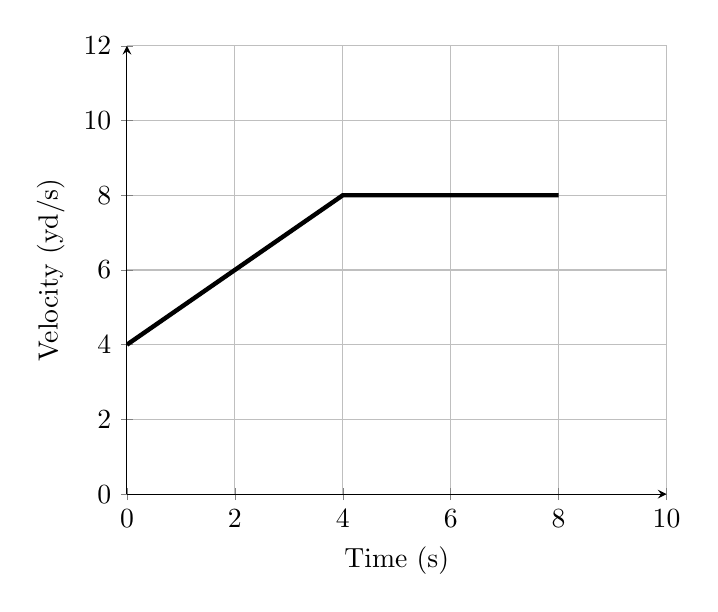
\begin{tikzpicture}
    \begin{axis}[axis y line=left, 
        axis x line=left,
        ymin=0, ymax=12,
        xmin=0, xmax=10,
        ylabel = Velocity (yd/s),
        xlabel = Time (s),
        grid=both,
        ytick={0,2,...,12}
    ]
    \addplot[
        %color=green!67!black,
        color=black,
        mark options={color=black},mark=none,
        ultra thick,
        ]
        coordinates {
        (0,4)
        (4,8)
        (8,8)
        };
    \end{axis}
    \end{tikzpicture}
    \label{fig:my_label}
\end{figure}

\question \label{prob:FootballPlayer1}
What is the player's \textbf{average acceleration} in the first 4 seconds?

\begin{choices}
\choice \SI{8}{yd/s^2}
\correctchoice \SI{1}{yd/s^2}
\choice \SI{4}{yd/s^2}
\choice \SI{2}{yd/s^2}
\end{choices}

\question \label{prob:FootballPlayer2}
What is the player's \textbf{average velocity} in the first 4 seconds?

\begin{choices}
\choice \SI{3}{yd/s}
\choice \SI{1}{yd/s}
\choice \SI{2}{yd/s}
\correctchoice \SI{6}{yd/s}
\end{choices}

\question \label{prob:FootballPlayer3}
If the player is at the 12-yard line at $t=0$, what is their \textbf{final position} at the end of the time interval?

\begin{choices}
\choice 64-yard line
\choice 8-yard line
\correctchoice 68-yard line
\choice 72-yard line
\end{choices}

\vspace{1em}
\hrule

\clearpage
\question
An object moves in accordance with the graph below. What is the object's acceleration?
\vspace{1em}

\begin{minipage}{0.3\textwidth}
    \begin{choices}
    \choice \SI{1}{m/s^2}
    \choice \SI{6}{m/s^2}
    \choice \SI{125}{m/s^2}
    \CorrectChoice \SI{5}{m/s^2}
    \end{choices}
\end{minipage}%
\begin{minipage}{0.3\textwidth}
\scalebox{0.8}{
    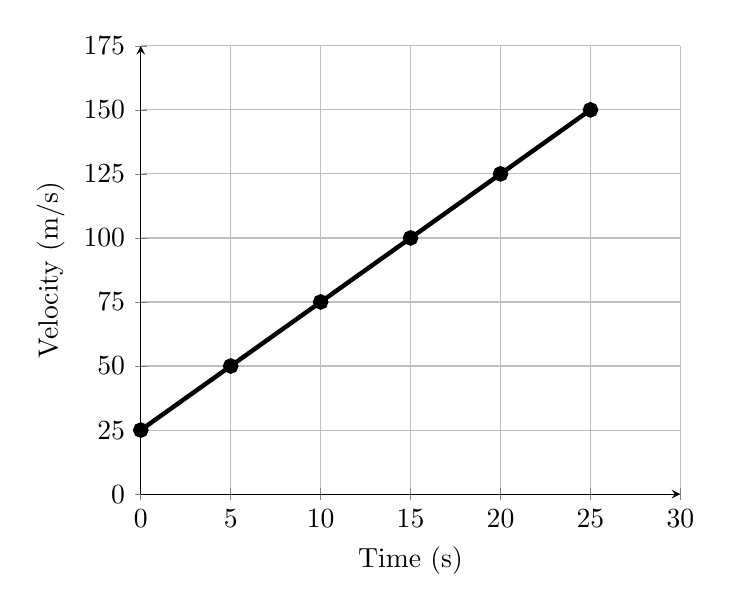
\begin{tikzpicture}
    \begin{axis}[axis y line=left, 
        axis x line=left,
        ymin=0, ymax=175,
        xmin=0, xmax=30,
        ylabel = Velocity (m/s),
        xlabel = Time (s),
        grid=both,
        ytick={0,25,...,175}
    ]
    \addplot[
        %color=green!67!black,
        color=black,
        mark options={color=black},mark=*,
        ultra thick,
        ]
        coordinates {
        (0,25)(5,50)(10,75)(15,100)(20,125)(25,150)
        };
    \end{axis}
    \end{tikzpicture}
    }
\end{minipage}




\clearpage


%%%%% END QUIZ 5 %%%%% END QUIZ 5 %%%%% END QUIZ 5 %%%%% END  QUIZ 5 %%%%% END QUIZ 5 %%%%%

%%%%% QUIZ 6 %%%%% QUIZ 6 %%%%% QUIZ 6 %%%%% QUIZ 6 %%%%% QUIZ 6 %%%%%


%\clearpage
% \question %Like Example 2.10 
% Dragsters can achieve average accelerations of \SI{23.0}{m/s^2}. Suppose such a dragster accelerates from rest at this rate for \SI{4.45}{s}. How far does it travel in this time?

% \begin{solutionorbox}[2in]

% $a = \SI{23.0}{m/s^2}$, $v_0 = 0$, $t = \SI{4.45}{s}$. Let $x_0 = 0$

% $x =\ ?$

% \begin{equation*}
%     x = x_0 + v_0 t + \frac{1}{2} a t^2 = \SI{228}{m}
% \end{equation*}
% \end{solutionorbox}

% \question %Like Ch2 #20
% An Olympic-class sprinter starts a race with an acceleration of \SI{4.30}{m/s^2}. What is her speed \SI{2.10}{s} later?

% \begin{solutionorbox}[2in]

% $a = \SI{4.30}{m/s^2}$, $t = \SI{2.10}{s}$, $v_0 = 0$

% $v =\ ?$

% \begin{equation*}
%     v = v_0 + at = \SI{9.03}{m/s}
% \end{equation*}


% \end{solutionorbox}

% %
% \question %Like Ch2 #27
% In a slap shot, a hockey player accelerates the puck from a velocity of \SI{5.70}{m/s} to \SI{88.4}{m/s} in the same direction. If this shot takes \SI{7.73e-2}{s}, calculate the distance over which the puck accelerates.

% \begin{solutionorbox}[2in]
% $v_0 = \SI{5.70}{m/s}$, $v = \SI{88.4}{m/s}$, $t = \SI{7.73e-2}{s}$. Let $x_0 = 0$.

% $x =\ ?$

% The average velocity is

% \begin{equation*}
%     \bar{v} = \frac{v_0 + v}{2} = \SI{47.0}{m/s}\ .
% \end{equation*}

% Therefore, distance traveled is

% \begin{equation*}
%     x = x_0 + \bar{v}t = \SI{3.64}{m}\ .
% \end{equation*}
% \end{solutionorbox}

% \question %Like Ch2 #28
% A powerful motorcycle can accelerate from rest to \SI{31.2}{m/s} in only \SI{4.23}{s}. How far does it travel in that time?

% \begin{solutionorbox}[2in]

% $v_0 = 0$ (``from rest''), $v = \SI{31.2}{m/s}$, $t = \SI{4.23}{s}$. Let $x_0 = 0$.

% $x =\ ?$

% Average velocity is

% \begin{equation*}
%     \bar{v} = \frac{v_0 + v}{2} = \SI{15.6}{m/s}\ .
% \end{equation*}

% Therefore, distance traveled is

% \begin{equation*}
%     x = x_0 + \bar{v}t = \SI{66.0}{m}\ .
% \end{equation*}

% \end{solutionorbox}

% \question %Like Ch2 #33
% An unwary football player collides with a padded goalpost while running at a velocity of \SI{6.13}{m/s} and comes to a full stop after compressing the padding and his body \SI{0.411}{m}. What is his deceleration?

% \begin{solutionorbox}[2in]

% $v_0 = \SI{6.13}{m/s}$, $v = 0$, $\Delta{x} = x - x_0 = \SI{0.411}{m}$. 

% $a =\ ?$

% The known and unknown quantities are related by the kinematic equation

% \begin{equation*}
%     v^2 = v^2_0 + 2 a \left(x - x_0\right)
% \end{equation*}

% Solving for acceleration leads to

% \begin{equation*}
%     a = \frac{v^2 - v_0^2}{2 \left(x - x_0\right)} = \SI{-45.7}{m/s^2}\ .
% \end{equation*}
% \end{solutionorbox}




\begin{EnvUplevel}
\textbf{Refer to the graph below and answer the questions below.}

\begin{center}
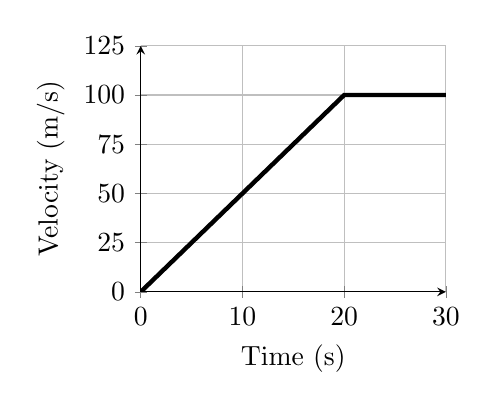
\begin{tikzpicture}
\begin{axis}[width=0.45\textwidth,
    axis y line=left, 
    axis x line=left,
    ymin=0, ymax=125,
    xmin=0, xmax=30,
    ylabel = Velocity (m/s),
    xlabel = Time (s),
    grid=both,
    ytick={0,25,...,175}
]
\addplot[
    %color=green!67!black,
    color=black,
    mark options={color=black},mark=none,
    ultra thick,
    ]
    coordinates {
    (0,0)(5,25)(10,50)(15,75)(20,100)(25,100)(30,100)
    };
\end{axis}
\end{tikzpicture}
\end{center}
\end{EnvUplevel}

\question
What is the \textbf{displacement} during the entire time interval?

\begin{solutionorbox}[2.5in]

For a \textbf{velocity vs.~time graph}, displacement is the area under the curve. 

\scalebox{0.8}{
\begin{tikzpicture}
\begin{axis}[color=black,axis y line=left, 
    axis x line=left,
    ymin=0, ymax=125,
    xmin=0, xmax=30,
    ylabel = Velocity (m/s),
    xlabel = Time (s),
    grid=both,
    ytick={0,25,...,175}
]

    \addplot[name path=f,domain=0:30,ultra thick,black] coordinates {(0,0)(20,100)(30,100)};

    \path[name path=axis] (axis cs:0,0) -- (axis cs:30,0);

    \addplot [
        thick,
        color=blue,
        fill=black!20!, 
        fill opacity=1
    ]
    fill between[
        of=f and axis,
        soft clip={domain=0:30},
    ];

\addplot[
    %color=green!67!black,
    color=black,
    mark options={color=black},mark=none,
    ultra thick,dashed,
    ]
    coordinates {
    (20,0)(20,100)
    };
\node at (axis cs:12,25) {\HUGE $A_1$};
\node at (axis cs:25,50) {\HUGE $A_2$};
\end{axis}
\end{tikzpicture}}

Dividing the graph at 20 seconds, the total area is composed of a right triangle of base \SI{20}{s} and height \SI{100}{m/s} ($A_1 = \frac{1}{2} \times \mathrm{base} \times \mathrm{height}$) and a rectangle of length \SI{10}{s} and width \SI{100}{m/s} ($A_2 = \mathrm{length} \times \mathrm{width}$).

Each area is

\begin{equation*}
    A_1 = \frac{1}{2}\left(\SI{20}{s}\right)\left(\SI{100}{m/s}\right) = \SI{1000}{m}
\end{equation*}

\begin{equation*}
    A_2 = (\SI{10}{s})(\SI{100}{m/s}) = \SI{1000}{m}
\end{equation*}

The total area, which equals the object's displacement, is

\begin{equation*}
    A = A_1 + A_2 = \SI{2000}{m}\ .
\end{equation*}

\end{solutionorbox}


\question
What is the \textbf{average velocity} during the first 20 seconds?

\begin{solutionorbox}[2.5in]

In the first 20 seconds, the corresponding initial and final velocities are $v_0 = 0$ and $v_f = \SI{100}{m/s}$. Average velocity under constant, non-zero acceleration is

\begin{equation*}
    \bar{v} = \frac{v_0 + v_f}{2} = \SI{50}{m/s}\ .
\end{equation*}

\end{solutionorbox}

\question %Like PCA
A skater starts at the top of a ramp and skates to the bottom. How is the skater's average acceleration calculated?

\begin{choices}
\CorrectChoice velocity at the \textbf{bottom} of the ramp \textit{minus} velocity at the \textbf{top}, \textit{divided} by the time it takes to reach the bottom
\choice velocity at the \textbf{top} of the ramp \textit{minus} velocity at the \textbf{bottom}, \textit{divided} by the time it takes to reach the bottom
\choice position at the \textbf{bottom} of the ramp \textit{minus} position at the \textbf{top}, \textit{divided} by the time it takes to reach the bottom
\choice position at the \textbf{top} of the ramp \textit{minus} position at the \textbf{bottom}, \textit{divided} by the time it takes to reach the bottom
\end{choices}


\question %Like PCA
An elevator moving down is slowing down. What is the direction of its acceleration?

\begin{choices}
\choice Left
\choice Right 
\choice Up
\correctchoice Down
\end{choices}

% \question %Like PCA
% A car moving to the right is speeding up. What is the direction of its acceleration?

% \question %Like PCA
% A car moving to the left is slowing down. What is the direction of its acceleration?

% \question %Like PCA
% A car moving to the left is speeding up. What is the direction of its acceleration?

% \question %Like PCA
% An elevator moving downward is slowing down. What is the direction of its acceleration?

% \question %Like PCA
% An elevator moving downward is speeding up. What is the direction of its acceleration?

% \begin{choices}
% \choice Up
% \choice Right
% \choice Left
% \CorrectChoice Down
% \end{choices}

% \question %Like PCA
% An elevator moving upward is slowing down. What is the direction of its acceleration?

% \question
% An elevator moving upward is speeding up. What is the direction of its acceleration?




\question % Like Ch2 #12
The driver of a sports car traveling at \SI{12.5}{m/s} steps down hard on the accelerator for \SI{4.5}{s} and the velocity increases to \SI{57.0}{m/s}. What was the average acceleration of the car during the \SI{4.5}{s} time interval?

\begin{choices}
\choice \SI{12.6}{m/s^2}
\choice \SI{2.7}{m/s^2}
\CorrectChoice \SI{9.9}{m/s^2}
\choice \SI{0.10}{m/s^2}
\end{choices}

\question % Like Ch2 #18
If a velocity increases from 0 to 36 m/s in 12 s, what is the average acceleration?

\begin{choices}
\choice \SI{0.333}{m/s^2}
\CorrectChoice \SI{3.0}{m/s^2}
\choice \SI{36}{m/s^2}
\choice \SI{432}{m/s^2}
\end{choices}

\question
What is average acceleration?

\begin{choices}
    \choice change in velocity divided by change in position
    \correctchoice change in velocity divided by change in time
    \choice rate of change of displacement
    \choice rate of change of position
\end{choices}

\question
Acceleration may be measured in units of \fillin\ .

\begin{choices}
    \choice meters per second (\SI{}{m/s})
    \correctchoice meters per second squared (\SI{}{m/s^2})
    \choice meters squared per second (\SI{}{m^2/s})
    \choice seconds (s)
\end{choices}

\question
If a falcon is flying at \SI{10}{m/s} and then, some short time later, flies at \SI{17}{m/s}, what is the falcon's change in velocity?

\begin{choices}
    \choice It's not possible to know without knowing the change in time.
    \choice \SI{10}{m/s}
    \choice \SI{17}{m/s}
    \correctchoice \SI{7.0}{m/s}
\end{choices}

\question
Amanda jogs with a constant velocity of \SI{6.2}{m/s} for 3.0 seconds. What is her average acceleration?

\begin{choices}
    \choice \SI{2.06}{m/s^2}
    \choice \SI{0.48}{m/s^2}
    \choice \SI{6.2}{m/s^2}
    \correctchoice \SI{0.0}{m/s^2}
\end{choices}

\question % Like Ch2 #18
The velocity of an airplane increases from 0 to \SI{36}{m/s} in \SI{12}{s}. What is the plane's average acceleration?

\begin{choices}
\choice \SI{0.333}{m/s^2}
\CorrectChoice \SI{3.0}{m/s^2}
\choice \SI{36}{m/s^2}
\choice \SI{432}{m/s^2}
\end{choices}

\question
An object moves in accordance with the graph below. What is the object's acceleration?
\vspace{1em}

\begin{minipage}{0.3\textwidth}
    \begin{choices}
    \choice \SI{1}{m/s^2}
    \choice \SI{6}{m/s^2}
    \choice \SI{125}{m/s^2}
    \CorrectChoice \SI{5}{m/s^2}
    \end{choices}
\end{minipage}%
\begin{minipage}{0.3\textwidth}
    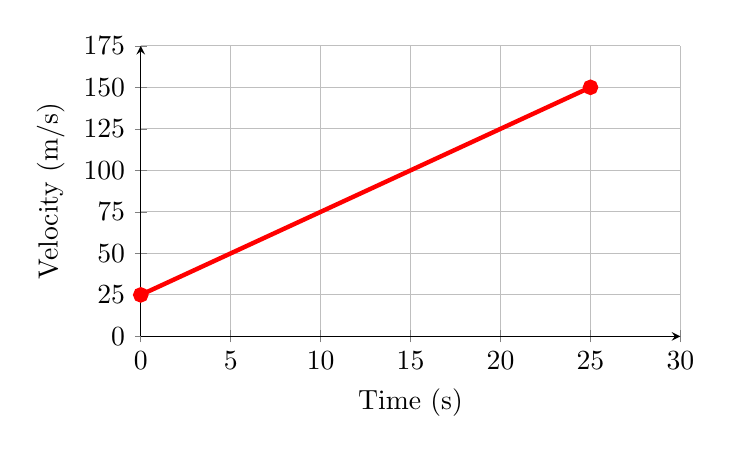
\begin{tikzpicture}
    \begin{axis}[width=240pt, height=150pt,
    axis y line=left, 
        axis x line=left,
        ymin=0, ymax=175,
        xmin=0, xmax=30,
        ylabel = Velocity (m/s),
        xlabel = Time (s),
        grid=both,
        ytick={0,25,...,175}
    ]
    \addplot[
        %color=green!67!black,
        color=red,
        mark options={color=red},mark=*,
        ultra thick,
        ]
        coordinates {
        (0,25)(25,150)
        };
    \end{axis}
    \end{tikzpicture}
\end{minipage}




\question
What is the acceleration of an object whose motion is shown by the graph below?

\begin{minipage}{0.3\textwidth}
    \begin{choices}
        \choice \SI{-52.5}{m/s^2}
        \choice \SI{3}{m/s^2}
        \choice \SI{52.5}{m/s^2}
        \correctchoice \SI{-3}{m/s^2}
    \end{choices}
\end{minipage}%
\begin{minipage}{0.3\textwidth}
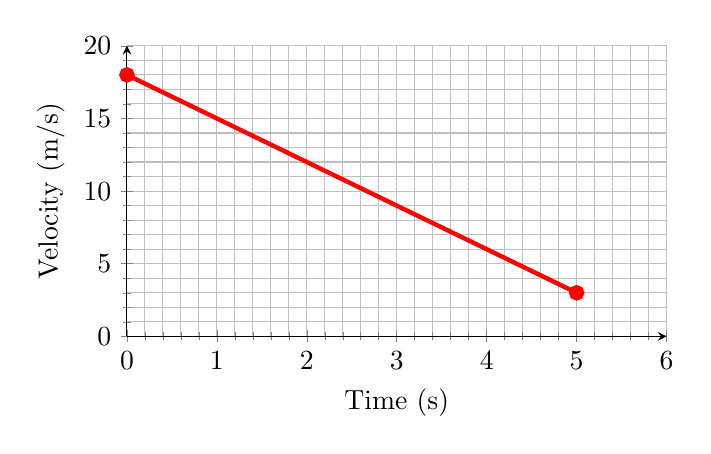
\begin{tikzpicture}
\begin{axis}[width=240pt, height=150pt,
        axis y line=left, 
        axis x line=left,
        ymin=0, ymax=20,
        xmin=0, xmax=6,
        ylabel = Velocity (m/s),
        xlabel = Time (s),
        grid=both,
        ytick={0,5,...,20},
        yminorgrids=true, minor y tick num=4,
        xminorgrids=true, minor x tick num=4,
    ]
    \addplot[
        color=red,
        mark options={color=red},mark=*,
        ultra thick,
        ]
        coordinates {
        (0,18)(5,3)
        };
\end{axis}
\end{tikzpicture} 
\end{minipage}

\question
Mario the soccer player jogs in one direction at a constant velocity in accordance with the graph below. What is his displacement?

\begin{minipage}{0.3\textwidth}
    \begin{choices}
        \choice \SI{0.0}{m}
        \correctchoice \SI{56}{m}
        \choice \SI{7}{m}
        \choice \SI{15}{m}
    \end{choices}
\end{minipage}%
\begin{minipage}{0.3\textwidth}
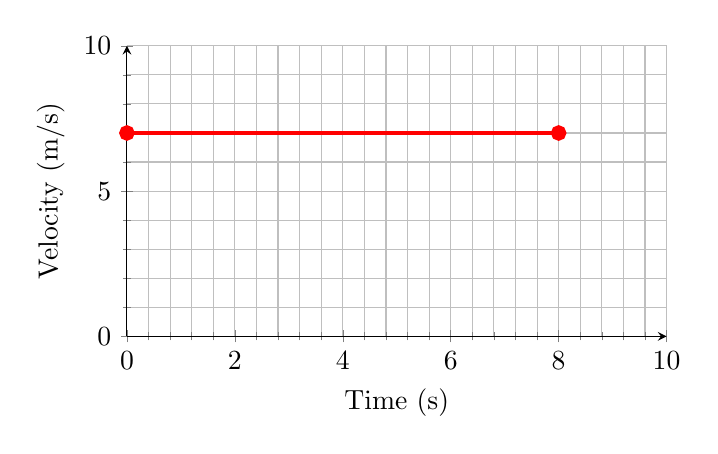
\begin{tikzpicture}
\begin{axis}[width=240pt, height=150pt,
        axis y line=left, 
        axis x line=left,
        ymin=0, ymax=10,
        xmin=0, xmax=10,
        ylabel = Velocity (m/s),
        xlabel = Time (s),
        grid=both,
        ytick={0,5,...,10},
        % ymajorgrids=true,
        % xmajorgrids=true,
        yminorgrids=true, minor y tick num=4,
        xminorgrids=true, minor x tick num=4,
    ]
    %\fill[black!20] (axis cs: 0,0) rectangle (axis cs: 6,15);
    \addplot[
        color=red,
        mark options={color=red},mark=*,
        ultra thick,
        ]
        coordinates {
        (0,7)(8,7)
        };
\end{axis}
\end{tikzpicture}
\end{minipage}

\question
An object's motion is represent by the graph below. What is the object's displacement?

\begin{minipage}{0.3\textwidth}
    \begin{choices}
        \correctchoice \SI{-15}{m}
        \choice \SI{15}{m}
        \choice \SI{-105}{m}
        \choice \SI{105}{m}
    \end{choices}
\end{minipage}%
\begin{minipage}{0.3\textwidth}
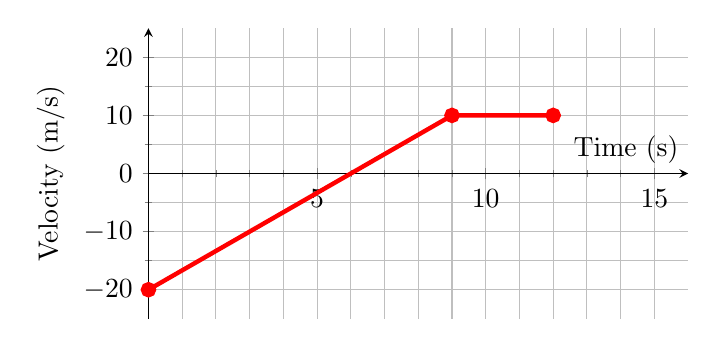
\begin{tikzpicture}
\begin{axis}[width=240pt,height=150pt,
    axis y line=left, 
    axis x line=center,
    xlabel = Time (s),
    ylabel = Velocity (m/s),
    ymin=-25, ymax=25,
    xmin=0, xmax=16,
    ytick={-20,-10,...,20},
    xtick={0,5,...,15},
    ymajorgrids=true,
    xmajorgrids=true,
    yminorgrids=true, minor y tick num=1,
    xminorgrids=true, minor x tick num=4,
    % x label style={anchor=west},
    clip=false,
]
    \addplot[
        %color=green!67!black,
        color=red,
        mark options={color=red},mark=*,
        ultra thick,
        ]
        coordinates {
        (0,-20)
        (9,10)
        (12,10)
        };
\end{axis}
\end{tikzpicture}
\end{minipage}

\end{questions}
\end{document}